\documentclass{standalone}
\usepackage{tikz}
\usepackage{pgfplots}
\pgfplotsset{width=32cm,height=18cm,compat=1.3}
\pgfplotsset{every tick label/.append style={font=\Huge}}
\usepackage{filecontents}

\usetikzlibrary{patterns}

\definecolor{citrine}{rgb}{0.89, 0.82, 0.04}

\begin{document}
	\centering
		\vspace{1.5em}
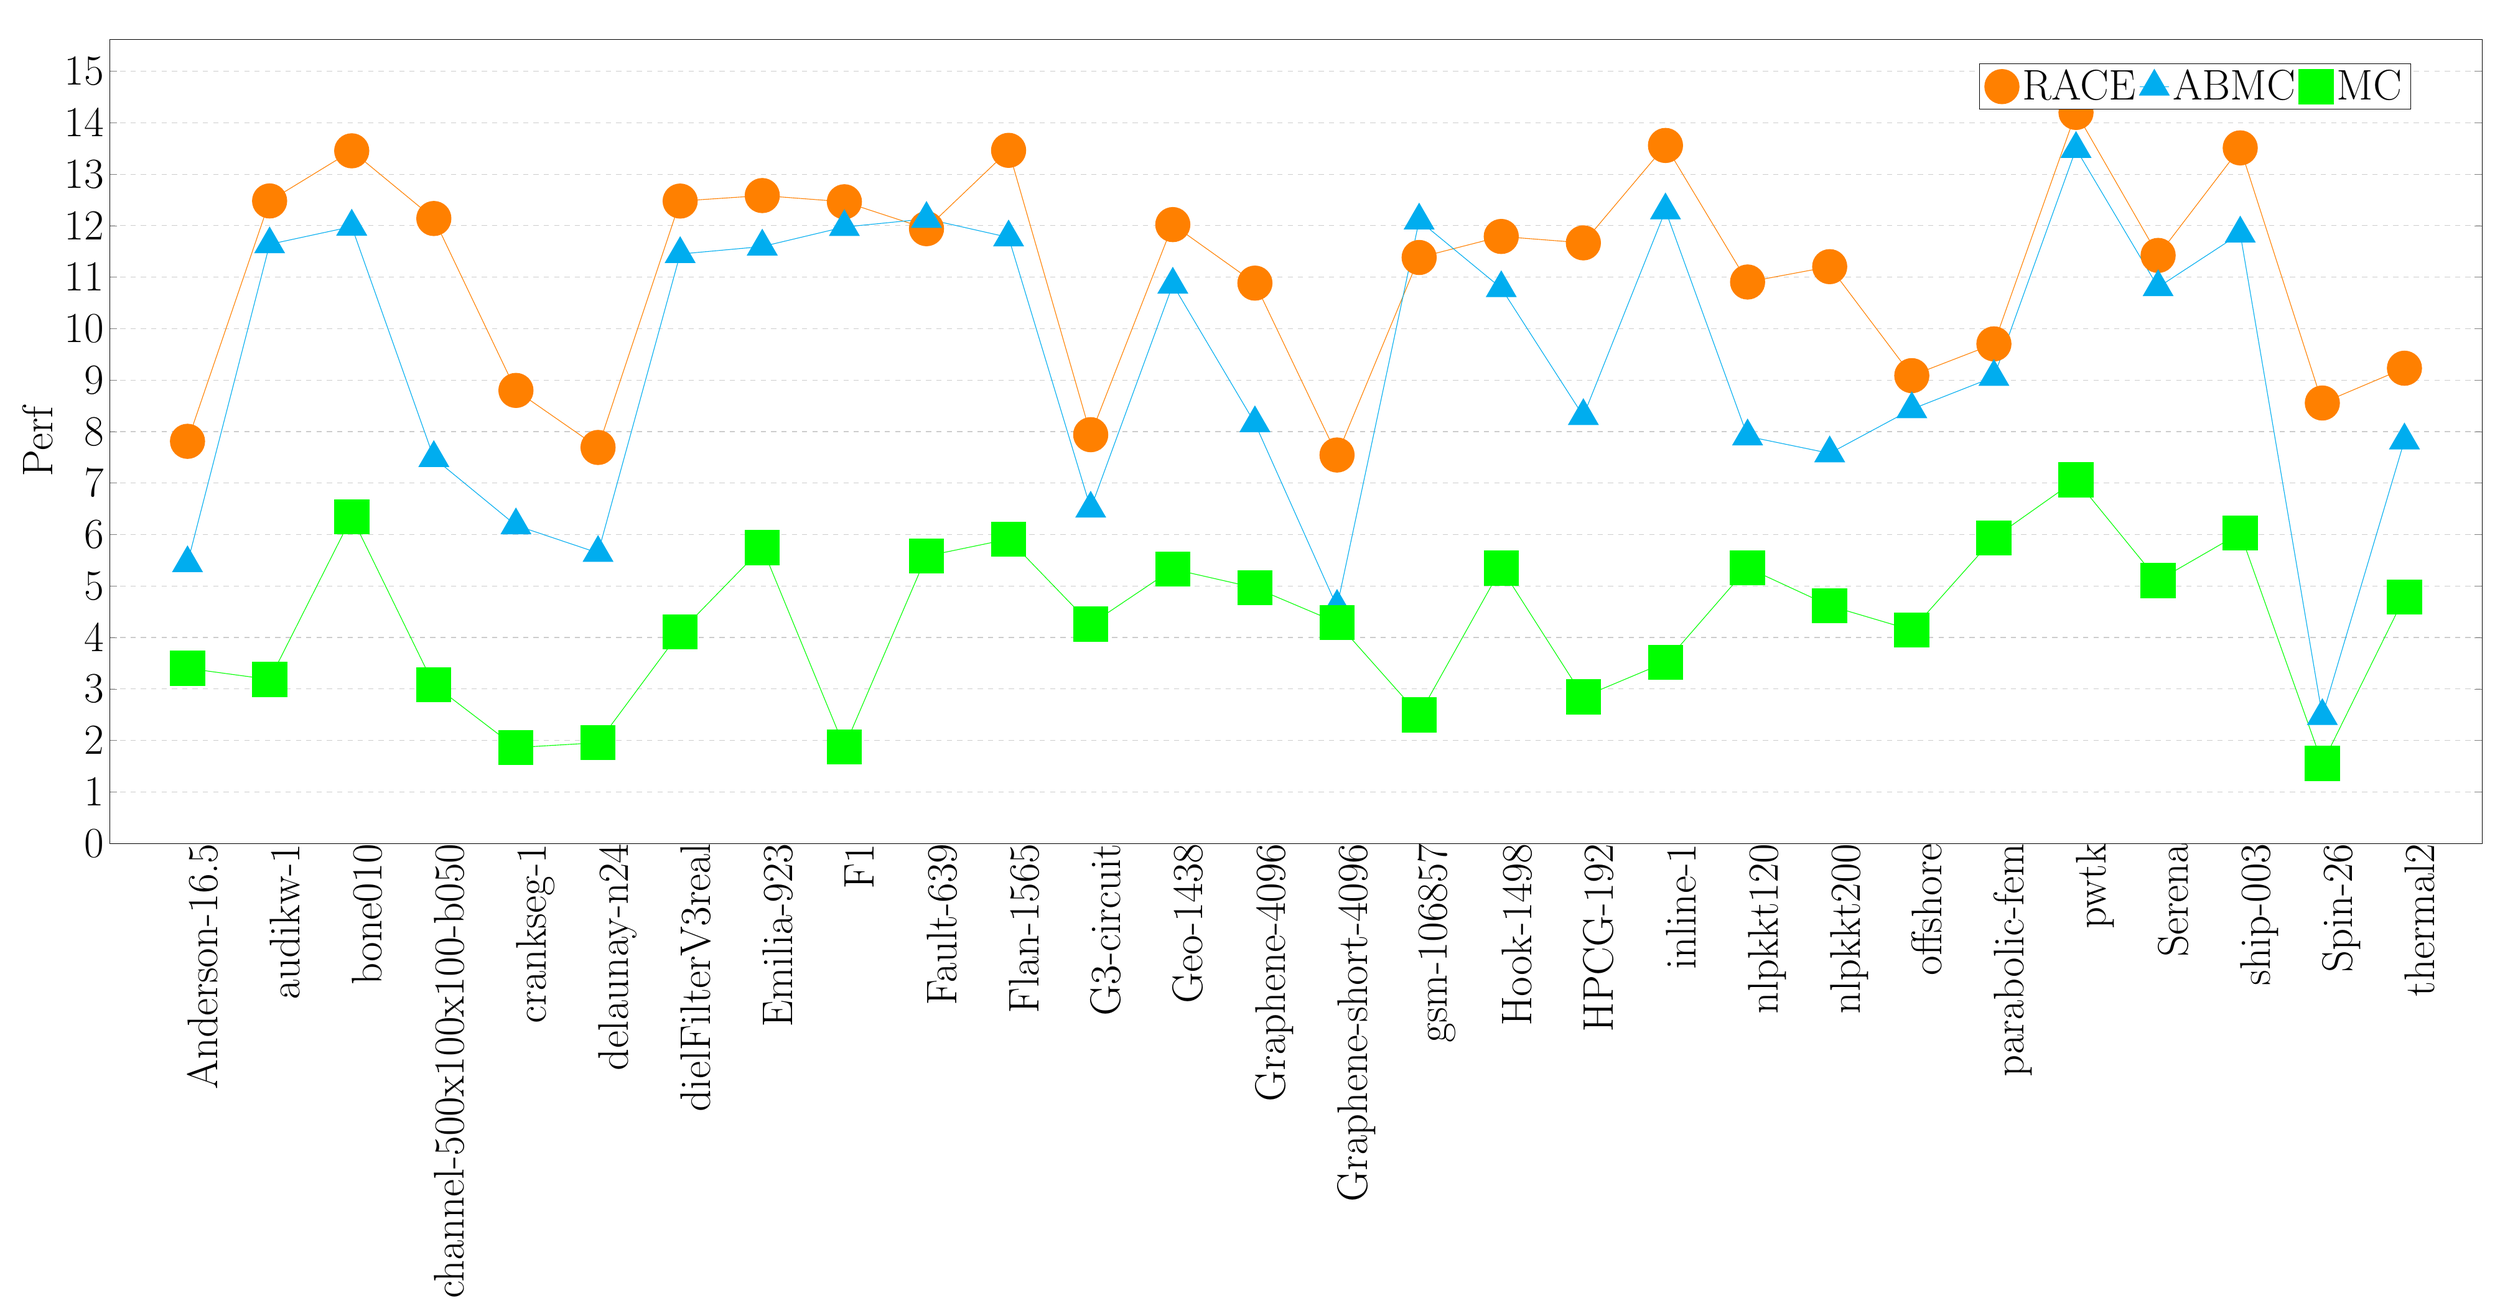
\begin{tikzpicture}
		%	\node at (13.25,15) {\LARGE{}};
			\begin{axis}[
		%	xmin=0.25, xmax=7.25,
			ymin=0, %ymax=3.25,
			xtick={1, 2, 3, 4, 5, 6, 7, 8, 9, 10, 11, 12, 13, 14, 15, 16, 17, 18, 19, 20, 21, 22, 23, 24, 25, 26, 27, 28},
		%	ytick={0,0.5,1,1.5,2,2.5,3},
			xticklabels={Anderson-16.5, audikw-1, bone010, channel-500x100x100-b050, crankseg-1, delaunay-n24, dielFilterV3real, Emilia-923, F1, Fault-639, Flan-1565, G3-circuit, Geo-1438, Graphene-4096, Graphene-short-4096, gsm-106857, Hook-1498, HPCG-192, inline-1, nlpkkt120, nlpkkt200, offshore, parabolic-fem, pwtk, Serena, ship-003, Spin-26, thermal2},
			width  = 50cm,
			height = 18cm,
			major x tick style = transparent,
			%	minor ytick={1, 5, 10, 15, 20, 25, 30 ,35,40},
			grid = minor,	
			%add_bar_commands
			ymajorgrids = true,
			grid style={dashed, gray!40},
			ylabel = {\Huge{Perf}},
		%	symbolic x coords={Graphene-2048-2048, Graphene-4096-4096, Spin-24-24-24},
			x tick label style={rotate=90, anchor=north east, inner sep=0mm, font={\Huge}},
			tick label style={font={\Huge}},
			scaled y ticks = false,
			enlarge x limits=0.035,
			legend cell align=left,
			legend style={font=\Huge},
			legend columns=-1,
			legend style={
				%at={(1,1.05)},
				%anchor=south east,
				%column sep=1ex,
				legend pos=north east
			},
			%spl_legend_code
			title= {\Huge\scalebox{1.5}{{}}}
			]

\addplot[mark=*, mark size=10pt, mark options={orange}, draw=orange ] plot coordinates{(1,7.811229) (2,12.481031) (3,13.454827) (4,12.139824) (5,8.799993) (6,7.691780) (7,12.478694) (8,12.585517) (9,12.464941) (10,11.942039) (11,13.463977) (12,7.939802) (13,12.021507) (14,10.884372) (15,7.545134) (16,11.382424) (17,11.791030) (18,11.666773) (19,13.559009) (20,10.906182) (21,11.204207) (22,9.087057) (23,9.703977) (24,14.200478) (25,11.422656) (26,13.511751) (27,8.555170) (28,9.231351)};
\addplot[mark=triangle*, mark size=10pt, mark options={cyan}, draw=cyan ] plot coordinates{(1,5.443401) (2,11.638545) (3,11.982375) (4,7.487216) (5,6.178656) (6,5.642745) (7,11.449803) (8,11.595278) (9,11.974533) (10,12.132818) (11,11.772924) (12,6.503159) (13,10.855085) (14,8.162013) (15,4.595417) (16,12.100507) (17,10.786634) (18,8.302103) (19,12.298856) (20,7.907156) (21,7.577819) (22,8.435306) (23,9.062039) (24,13.491702) (25,10.805083) (26,11.847884) (27,2.473984) (28,7.829024)};
\addplot[mark=square*, mark size=10pt, mark options={green}, draw=green ] plot coordinates{(1,3.400937) (2,3.184375) (3,6.343043) (4,3.080497) (5,1.861477) (6,1.956021) (7,4.107050) (8,5.743727) (9,1.871931) (10,5.580948) (11,5.911824) (12,4.257442) (13,5.329090) (14,4.966167) (15,4.290495) (16,2.495243) (17,5.347373) (18,2.847961) (19,3.517903) (20,5.354115) (21,4.616286) (22,4.143928) (23,5.934224) (24,7.061438) (25,5.108226) (26,6.027780) (27,1.552193) (28,4.783377)};
	%addplot cmd

	\legend{RACE, ABMC, MC}

	\end{axis}			
\end{tikzpicture}

\end{document}

